All code and results for this project is available online at:\\
\hreftt{https://github.com/mishra-lab/covid19-Re}
\par
Table~\ref{tab:distr} summarizes
the reported parametric \covid distributions, and
Figure~\ref{fig:distr-refs} illustrates
the serial interval and generation time distributions
explored for estimating $\Re(t)$.
Figure~\ref{fig:Re-zoom} provides a zoom-in of
Figure~\ref{fig:Re} after March 30.
\par
\begin{table}[h]
  \caption{Summary of reported parametric \covid distributions}
  \centering
{\small
\begin{tabular}{rlrlll}
	\toprule
	          & Ref                 &   $N$ & Distribution                           & Mean   & SD     \\
	\midrule
	$S(\tau)$ & \citet{Du2020}       & $468$ & $\op{Norm}{\mu=3.96,~\sigma=4.75}$     & $3.96$ & $4.75$ \\
	          & \citet{Zhang2020}    &  $35$ & $\op{Gam}{\alpha=3.619,~\beta=1.416}$  & $5.1$  & $2.7$  \\
	          & \citet{Nishiura2020} &  $28$ & $\op{LogN}{\mu=4.7,~\sigma=2.9}$       & $4.7$  & $2.9$  \\
	          & \citet{Zhao2020}     &  $21$ & $\op{Gam}{\alpha=2.151,~\beta=2.045}$  & $4.4$  & $3.0$  \\
	          & \citet{Li2020}       &   $6$ & $\op{Gam}{\alpha=4.866,~\beta=1.541}$  & $7.5$  & $3.4$  \\
	          & \citet{Tindale2020}  &   $4$ & $\op{Norm}{\mu=4.22,~\sigma=0.4}$      & $4.22$ & $0.4$  \\
	          & \citet{Tindale2020}  &   $4$ & $\op{Norm}{\mu=4.56,~\sigma=0.95}$     & $4.56$ & $0.95$ \\
	\midrule
	$H(\tau)$ & \citet{Lauer2020}    & $181$ & $\op{Gam}{\alpha=5.807,~\sigma=0.948}$ & $5.51$ & $2.28$ \\
	          & \citet{Tindale2020}  & $135$ & $\op{Weib}{\alpha=2.25,~\beta=10.15}$  & $8.99$ & $4.23$ \\
	          & \citet{Tindale2020}  &  $93$ & $\op{Weib}{\alpha=1.88,~\beta=7.97}$   & $7.07$ & $3.91$ \\
	          & \citet{Linton2020}   &  $52$ & $\op{LogN}{\mu=5.6,~\sigma=2.8}$       & $5.6$  & $2.8$  \\
	          & \citet{Backer2020}   &  $88$ & $\op{Weib}{\alpha=3.038,~\beta=7.163}$ & $6.4$  & $2.3$  \\
	          & \citet{Li2020}       &  $10$ & $\op{LogN}{\mu=5.2,~\sigma=3.91}$      & $5.2$  & $3.91$ \\
	\midrule
	$G(\tau)$ & this                 &   --- & $\op{Gam}{\alpha=1.633,~\beta=2.498}$  & $4.08$ & $3.19$ \\
	          & \citet{Ganyani2020}  &     * & $\op{Gam}{\alpha=9.140,~\beta=0.569}$  & $5.20$ & $1.72$ \\
	          & \citet{Ganyani2020}  &     * & $\op{Gam}{\alpha=6.843,~\beta=0.577}$  & $3.95$ & $1.51$ \\
	\bottomrule
\end{tabular}}
\floatfoot{
  Notation ---
  $N$: sample size;
  *: indeterminate;
  $S(\tau)$: serial interval;
  $H(\tau)$: incubation time;
  $G(\tau)$: generation time;
  $\mu$: mean;
  $\sigma$: std dev (\sd);
  $\alpha$: shape;
  $\beta$: scale.
  Notes ---
  some parameters were back-calculated based on
  reported distribution statistics like mean, \sd, and quantiles;
  $\mathrm{LogN}$ mean and \sd are in linear, not log scale.
}
  \label{tab:distr}
\end{table}
\par
\begin{figure}[h]
  \centering
  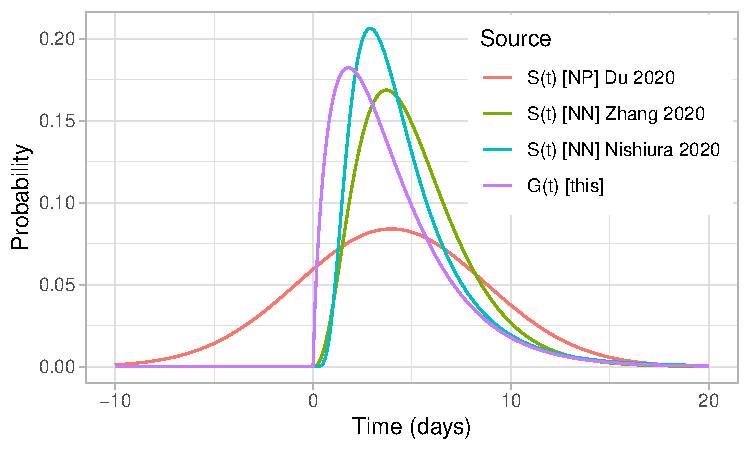
\includegraphics[width=\linewidth]{distr-refs}
  \caption{Illustration of reported serial interval and generation time
    distributions used for calculating $\Re(t)$ in \covid}
  \label{fig:distr-refs}
\end{figure}
\par
\begin{figure}[h]
  \centering
  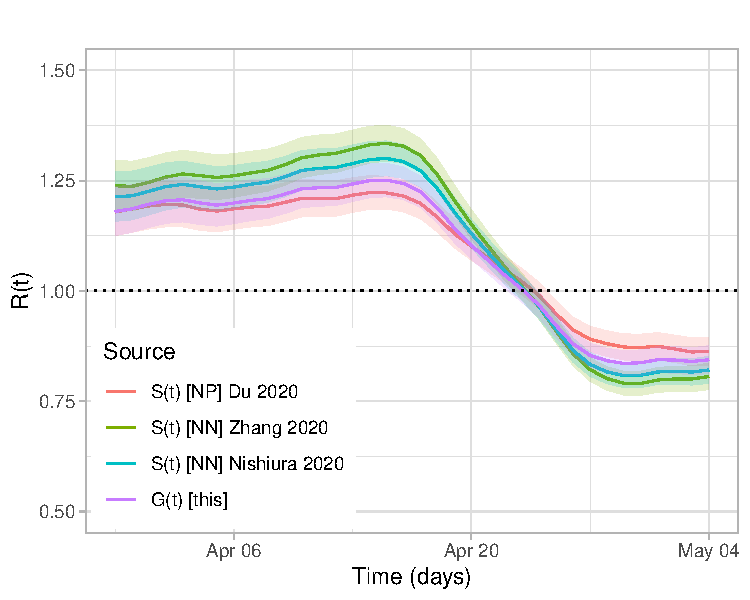
\includegraphics[width=\linewidth]{Re-zoom}
  \caption{$\Re(t)$ of \covid in \gta using
    serial interval versus generation time
    (zoom of March 30 to May 4)}
  \label{fig:Re-zoom}
  \floatfoot{Notation ---
    $S(\tau)$:~serial interval;
    $G(\tau)$:~generation time;
    [NP]:~negative-permitting;
    [NN]:~non-negative.
  }
\end{figure}